% ============================================================================
%  TAE (Trust-AI-Eval) @ NeurIPS 2026 -- workshop submission (double-blind)
%  Build:  latexmk -pdf tae_workshop.tex
%  Camera-ready: change the package option to [dblblindworkshop, final]
%  Note: the paper labels the evaluator factor D (distortion). The result files
%  and code key the same factor E; docs/CLAIM_REGISTRY.md records the mapping.
% ============================================================================
\documentclass{article}

\usepackage[dblblindworkshop]{neurips_2026}
\workshoptitle{TAE (Trust-AI-Eval): Can We Trust AI Evaluation?}

% The official style prints the same generic notice for every non-final submission, whatever the
% track, so a workshop submission is indistinguishable from a main-conference one. The workshop
% option IS set above; this preamble override (no style file is modified) makes the track visible to
% reviewers, exactly as the [final] build would.
\makeatletter
\renewcommand{\@noticestring}{%
  Submitted to the \@neuripsordinal\/ Conference on Neural Information Processing Systems
  (NeurIPS \@neuripsyear). Workshop: \@workshoptitle\ Do not distribute.%
}
\makeatother

\usepackage[utf8]{inputenc}
\usepackage[T1]{fontenc}
\usepackage{hyperref}
\usepackage{url}
\usepackage{booktabs}
\usepackage{amsmath,amssymb,amsfonts,amsthm}
\usepackage{nicefrac}
% expansion=false: pdftex (TeX Live 2026) aborts in pdfvlistout when hyperref link annotations
% coexist with font expansion in this document. Protrusion is kept.
\usepackage[expansion=false]{microtype}
\usepackage{xcolor}
\usepackage{graphicx}
\usepackage{enumitem}

\theoremstyle{plain}
\newtheorem{proposition}{Proposition}[section]
\newtheorem{corollary}[proposition]{Corollary}
\theoremstyle{remark}
\newtheorem{remark}[proposition]{Remark}

\newcommand{\Yref}{Y^{\mathrm{ref}}}
\newcommand{\muref}{\mu^{\mathrm{ref}}}
\newcommand{\muop}{\mu^{\mathrm{op}}}
\newcommand{\Bsel}{B^{\mathrm{sel}}}
\newcommand{\Rref}{R^{\mathrm{ref}}}
\newcommand{\piref}{\pi^{\mathrm{ref}}}
\newcommand{\Gsel}{G_{\mathrm{sel}}}
\newcommand{\Gmeas}{G_{\mathrm{meas}}}
\newcommand{\se}[1]{{\scriptstyle\pm#1}}

% auto-generated by code/make_tae_artifacts.py -- do not edit by hand
\newcommand{\TAEdeploymentrows}{%
\multicolumn{7}{@{}l}{\emph{A1--D1 (stable evaluator distortion)}}\\
CASE, ungated & $0.0338{\scriptstyle\pm0.0017}$ & $0.178{\scriptstyle\pm0.030}$ & $0.000{\scriptstyle\pm0.000}$ & 0.99 & 13\,/\,0 & --\\
\;$+$ same-evaluator check & $0.0374{\scriptstyle\pm0.0020}$ & $0.061{\scriptstyle\pm0.019}$ & $0.233{\scriptstyle\pm0.039}$ & 0.56 & 9\,/\,4 & $4.6\%$\\
\;$+$ reference-channel check & $0.0373{\scriptstyle\pm0.0020}$ & $0.072{\scriptstyle\pm0.021}$ & $0.233{\scriptstyle\pm0.038}$ & 0.57 & 9\,/\,4 & $0.0\%$\\
\addlinespace[2pt]
\multicolumn{7}{@{}l}{\emph{A1--D2 (evaluator differs between log and audit)}}\\
CASE, ungated & $0.0348{\scriptstyle\pm0.0020}$ & $0.189{\scriptstyle\pm0.034}$ & $0.000{\scriptstyle\pm0.000}$ & 0.99 & 13\,/\,0 & --\\
\;$+$ same-evaluator check & $0.0379{\scriptstyle\pm0.0020}$ & $0.050{\scriptstyle\pm0.016}$ & $0.244{\scriptstyle\pm0.036}$ & 0.52 & 9\,/\,4 & $4.8\%$\\
\;$+$ reference-channel check & $0.0377{\scriptstyle\pm0.0019}$ & $0.078{\scriptstyle\pm0.021}$ & $0.239{\scriptstyle\pm0.035}$ & 0.56 & 9\,/\,4 & $0.0\%$\\
\addlinespace[2pt]
}
\newcommand{\TAEfactorialrows}{%
A0--D0 & $0.0214{\scriptstyle\pm0.0024}$ & $0.0338{\scriptstyle\pm0.0021}$ & $0.0321{\scriptstyle\pm0.0024}$ & $0.0326{\scriptstyle\pm0.0024}$ & $0.0000{\scriptstyle\pm0.0000}$ & $0.0000{\scriptstyle\pm0.0000}$\\
A1--D0 & $0.0499{\scriptstyle\pm0.0030}$ & $0.0414{\scriptstyle\pm0.0022}$ & $0.0338{\scriptstyle\pm0.0020}$ & $0.0335{\scriptstyle\pm0.0019}$ & $0.0000{\scriptstyle\pm0.0000}$ & $0.0000{\scriptstyle\pm0.0000}$\\
A0--D1 & $0.0245{\scriptstyle\pm0.0024}$ & $0.0326{\scriptstyle\pm0.0019}$ & $0.0330{\scriptstyle\pm0.0021}$ & $0.0325{\scriptstyle\pm0.0019}$ & $0.0030{\scriptstyle\pm0.0006}$ & $0.0000{\scriptstyle\pm0.0000}$\\
A1--D1 & $0.0469{\scriptstyle\pm0.0025}$ & $0.0414{\scriptstyle\pm0.0023}$ & $0.0338{\scriptstyle\pm0.0017}$ & $0.0350{\scriptstyle\pm0.0016}$ & $0.0030{\scriptstyle\pm0.0006}$ & $0.0000{\scriptstyle\pm0.0000}$\\
}
\newcommand{\TAEslicerows}{%
\multicolumn{7}{@{}l}{\emph{A1--D0}}\\
Trust log & $0.0711$ & $0.0239$ & $0.0359$ & $0.0535$ & $0.1311$ & $0.0631$\\
Uniform audit & $0.0528$ & $0.0112$ & $0.0249$ & $0.0624$ & $0.0815$ & $0.0466$\\
Raw margin, obs.\ surface & $0.0526$ & $0.0115$ & $0.0259$ & $0.0541$ & $0.0911$ & $0.0470$\\
R-EPIG, obs.\ surface & $0.0532$ & $0.0127$ & $0.0246$ & $0.0523$ & $0.0864$ & $0.0458$\\
CASE, deconf.\ surface & $0.0407$ & $0.0131$ & $0.0223$ & $0.0502$ & $0.0741$ & $0.0401$\\
R-EPIG, deconf.\ surface & $0.0430$ & $0.0142$ & $0.0231$ & $0.0483$ & $0.0751$ & $0.0407$\\
\addlinespace[2pt]
\multicolumn{7}{@{}l}{\emph{A1--D1}}\\
Trust log & $0.0581$ & $0.0217$ & $0.0356$ & $0.0619$ & $0.1217$ & $0.0598$\\
Uniform audit & $0.0502$ & $0.0113$ & $0.0252$ & $0.0690$ & $0.0840$ & $0.0479$\\
Raw margin, obs.\ surface & $0.0494$ & $0.0132$ & $0.0240$ & $0.0532$ & $0.0903$ & $0.0460$\\
R-EPIG, obs.\ surface & $0.0524$ & $0.0129$ & $0.0239$ & $0.0574$ & $0.0900$ & $0.0473$\\
CASE, deconf.\ surface & $0.0375$ & $0.0122$ & $0.0228$ & $0.0562$ & $0.0817$ & $0.0421$\\
R-EPIG, deconf.\ surface & $0.0420$ & $0.0135$ & $0.0244$ & $0.0544$ & $0.0822$ & $0.0433$\\
\addlinespace[2pt]
}


\title{Can We Trust Logged LLM Comparisons?\\Auditing Selection and Measurement Validity under Model Routing}

\author{Anonymous authors\\Paper under double-blind review}

\begin{document}
\maketitle

\begin{abstract}
Many AI products choose among several language models for each user request. A router may send
routine questions to a cheaper model and difficult questions to a stronger one, leaving a log of the
request, the model that answered it, and an automatic score. Teams use these logs to compare models
and decide which should handle each kind of request. We argue that such comparisons can fail in two
ways, while existing work largely addresses only one. Assignment validity fails when models are
judged on different requests. If one model receives harder questions, their average scores are not
directly comparable. Measurement validity fails when the score rewards the wrong thing. A grader may
prefer longer or more polished answers when the team cares about correctness or user value. Methods
for confounded logs use randomized audits to address the first problem, but usually treat the score
as valid. Research on evaluator bias studies the second problem, but rarely connects it to model
selection decisions from routed logs. We show that a randomized audit isolates routing bias only when
the grader makes the same average errors on routed and randomly selected requests. Even then, grader
bias remains. We test both failures on two public routing benchmarks. Auditing reduces assignment
bias on both, but not measurement bias. Under a prespecified scoring bias stress test, even perfect
routing correction selects the wrong model in $14$ to $18\%$ of request types on the two corpora, and
in $10$ to $31\%$ across our sensitivity analyses. We also find
that corrected scores matter more than the exact audit allocation rule, although the rule matters
more as the number of models grows. Finally, the first few randomized measurements can indicate
whether a larger audit is worthwhile.
\end{abstract}

% =============================================================================
\section{Introduction}\label{sec:intro}
% =============================================================================
A team runs a product on several language models behind a router, so that cheap models take the
routine traffic and expensive ones take the hard traffic
\citep{chen2023frugalgpt,ding2024hybrid,ong2024routellm}. After a month there is a log with millions
of rows, each holding a request, the model that served it, and an automatic score. Someone asks a
reasonable question. \emph{For coding requests, which model is best?} The log answers instantly and
for free, and the team switches coding traffic accordingly. That answer can be wrong for two reasons
that look alike and are not.

\paragraph{The models sat different exams (assignment validity).} The router decided which model saw
which request, and it decided on difficulty. Modern routers make this explicit. They predict per
request how well each candidate would do, or how uncertain it is, and escalate accordingly
\citep{feng2025graphrouter,zhang2025routerr1,su2026cprouter,zheng2026disrouter}. The strong model's
average is therefore taken over hard requests and the cheap model's over easy ones, so comparing the
averages compares models and exam papers at once. Recent work on routing supervision makes the same
observation from the training side, noting that outcomes sampled under a routing policy are a biased
view of a model's capability \citep{routing2026supervision}. This is the classic confounded-log
problem, and randomization is its classic answer.

\paragraph{The exam measured the wrong thing (measurement validity).} The score in the log came from
an automatic evaluator, such as an LLM acting as judge, a string-match grader, or a click-through
proxy. Such evaluators have documented systematic preferences, including for their own outputs, for
longer answers, and for whichever answer appears first
\citep{wang2024notfair,panickssery2024selfpreference,zheng2023judging,chiang2024arena}. If the
evaluator's ranking differs from the ranking the deployment decision is about, every model sat the
same exam and the exam was the wrong one. This is the classic \emph{construct}-validity question
\citep{jacobs2021measurement,raji2021everything}, namely whether the number you measured is the
quantity you care about, and randomizing who is graded on what does not touch it.

\paragraph{What is missing.} Both failures are individually familiar. The methods literature on
confounded logs combines an observational log with a small randomized sample and spends an
experimental budget where it changes decisions
\citep{athey2020combining,kallus2018removing,rosenman2018combining}, and the last two years have
sharpened both halves, with cross-validated fusion of experimental and observational data
\citep{yang2025crossvalidated}, confounding-robust offline learning that buys online interventions
\citep{li2025confounding}, and decision-oriented active designs
\citep{cha2025abc3,gao2025causalepig,gao2026observationally,gao2026budgeted}. All of it targets the
first failure and reports gains against a benchmark score treated as valid. The evaluation literature
documents the second, mostly by measuring judges against human labels, without connecting it to a
model-selection decision taken from a routed log. Missing is the joint statement a practitioner
needs, namely \emph{which} failure an audit repairs, what it leaves behind, and how the leftover
shows up in the decision they make. Answering that requires switching one failure on and off while
holding the other fixed, which no observational study of a production log can do and a controlled
replay of a released benchmark matrix can.

\paragraph{Contributions.}
\begin{enumerate}[leftmargin=1.4em,itemsep=1pt,topsep=2pt]
\item A decomposition (Prop.~\ref{prop:decomp}) that separates the two failures and, more usefully,
states the condition under which the standard repair is valid. The randomized-audit repair works only
if the evaluator's average error on the router's requests matches its average error on the general
population. Using the same judge on both is \emph{not} sufficient.
\item A crossed experiment that switches each failure on and off independently on the same data,
holding model roster, requests, contexts and log volume fixed, replicated end to end on a second
released matrix with a different roster.
\item Findings a practitioner can act on, covering what an audit repairs and what it cannot, why
deconfounding the surface the budget is spent on matters more than the acquisition rule but not
without limit, a usable test for whether an audit is worth buying, and the loss asymmetry at which a
deployment gate starts to pay.
\end{enumerate}

% =============================================================================
\section{Setup and notation}\label{sec:setup}
% =============================================================================
Consider a team that sends routine requests to a cheaper model and difficult requests to a stronger
one. We label each request by $i$ and group similar requests into $J$ contexts, where each context
represents a request type such as routine questions or difficult coding questions. The contexts are
numbered $j=1,\dots,J$, and $Z_i\in\{1,\dots,J\}$ records the context of request $i$. The team
compares $K$ candidate models, numbered $k=1,\dots,K$. For each logged request $i$,
$A_i\in\{1,\dots,K\}$ records which model answered it. Pairing model $k$ with context $j$ gives a
model and context cell, written as $(k,j)$, so there are $K\times J$ cells in total. A deployment
policy $\pi$ chooses one model for each context. Thus $\pi(j)=k$ means that the policy sends requests
in context $j$ to model $k$, so three models across four request types give twelve cells.

\paragraph{The outcome the decision is about.} Suppose the team wants to choose the model that
provides the greatest value for each type of request. We call this value the target outcome. For
request $i$ and model $k$, $\Yref_i(k)$ is the target outcome that model $k$ would receive if it
answered request $i$. In our experiments this is a released benchmark score, and in a deployment it
could be any measure fixed in advance, such as correctness or user satisfaction.
For model $k$ and context $j$, $\muref_{kj}=\mathbb E[\Yref_i(k)\mid Z_i=j]$ is the model's
average target outcome on requests in that context. The target policy, written $\piref$, assigns each
context to the model with the highest average target outcome. Thus
$\piref(j)=\arg\max_k \muref_{kj}$. We call this a designated target rather than ground truth because
it is the objective the team has chosen, and all results below ask whether the logged evaluation
recovers the decisions that objective implies.

\begin{table}[t]\centering\footnotesize\setlength{\tabcolsep}{5pt}
\caption{Notation. The three surfaces differ only in \emph{who was measured} and \emph{what the
measurement was}, and keeping them apart is the whole argument.}
\label{tab:notation}
\begin{tabular}{@{}llp{7.4cm}@{}}
\toprule
Symbol & Name & What it is\\
\midrule
$\muref_{kj}$ & target surface & average designated outcome of model $k$ on context-$j$ requests\\
$M_{kj}$ & logged surface & average \emph{recorded score} of model $k$ over the context-$j$ requests \emph{the router sent it}\\
$R_{kj}$ & audit readout & average recorded score of model $k$ on a fresh \emph{random} sample of context-$j$ requests\\
$\muop_{kj}$ & population-operational surface & what the evaluator would report for model $k$ on \emph{all} context-$j$ requests, with selection removed and evaluator error kept\\
$\Bsel_{kj}$ & selection bias & how much easier or harder the router's requests were, in target units\\
$C_{kj}$ & evaluator distortion & how far the recorded score sits from the target outcome, per cell\\
$\Delta_j$ & target margin & gap between best and second-best model in context $j$, under $\muref$\\
$\Rref(\pi)$ & deployment regret & target value lost by deploying $\pi$ instead of $\piref$, averaged over contexts\\
\bottomrule
\end{tabular}
\end{table}

\paragraph{Three streams, one evaluator.} The same evaluator scores requests in three data sources.
The observational log ($s=o$) contains requests after the router has chosen which model answers them,
the randomized audit ($s=i$) scores models on randomly selected requests, and the held-out
verification set ($s=v$) is kept apart and used only to check a final deployment decision. For
request $i$, model $k$, and data source $s$, $\widetilde Y^s_i(k)$ is the
score reported by the evaluator. Its error is the difference between this score and the target
outcome, $\widetilde Y^s_i(k)-\Yref_i(k)$. Even when the same evaluator is used, its average error may
differ between the log and the audit because the router chooses which requests each model receives in
the log. For model $k$ and context $j$, $C^{o,\mathrm{sel}}_{kj}$ is the evaluator's average error on
the requests in context $j$ that the router sent to model $k$, while $C^{i,\mathrm{pop}}_{kj}$ is its
average error when model $k$ is evaluated on a random sample of all requests in that context.
Formally,
\[
C^{o,\mathrm{sel}}_{kj}=\mathbb E\!\left[\widetilde Y^o_i(k)-\Yref_i(k)\mid A_i{=}k,Z_i{=}j\right],
\qquad
C^{i,\mathrm{pop}}_{kj}=\mathbb E\!\left[\widetilde Y^i_i(k)-\Yref_i(k)\mid Z_i{=}j\right].
\]
Finally, $\Bsel_{kj}=\mathbb E[\Yref_i(k)\mid A_i{=}k,Z_i{=}j]-\muref_{kj}$ measures the selection
bias created by the router, comparing how well model $k$ would perform on the requests it was
assigned with how well it would perform on all requests in context $j$. A positive value means the
router gave it more favorable requests and a negative value harder ones.
Table~\ref{tab:notation} summarizes the notation.

% =============================================================================
\section{What a randomized audit can and cannot repair}\label{sec:model}
% =============================================================================
A randomized audit gives each model a fairer sample of requests, so it can help separate model
quality from the router's assignment choices, but the correction is valid only under a specific
condition. Proposition~\ref{prop:decomp} splits the difference between the logged score and the audit
score into two parts, the selection bias created by the router and any change in the evaluator's
average error between the routed and the randomly sampled requests. The audit recovers selection
bias only when the second part is zero.

\begin{proposition}[Validity decomposition]\label{prop:decomp}
Up to sampling noise,
$
M_{kj}-R_{kj}=\Bsel_{kj}+\bigl(C^{o,\mathrm{sel}}_{kj}-C^{i,\mathrm{pop}}_{kj}\bigr).
$
Hence \emph{(a)} the logged-minus-audit difference recovers $\Bsel_{kj}$ exactly when
$C^{o,\mathrm{sel}}_{kj}=C^{i,\mathrm{pop}}_{kj}$, a condition we call \emph{assignment invariance},
meaning that the evaluator's mean error on the requests the router sent to model $k$ equals its mean
error on all context-$j$ requests. \emph{(b)} A sufficient condition is that the same evaluator scores
both streams \emph{and} its error depends on a request only through its cell, so that
$C^{o,\mathrm{sel}}_{kj}=C^{i,\mathrm{pop}}_{kj}=C_{kj}$. Subtracting the recovered difference from
$M$ then gives a surface targeting $\muop_{kj}=\muref_{kj}+C_{kj}$ rather than $\muref_{kj}$. In
particular a context-invariant model preference $C_{kj}=C_k$ cancels from the difference entirely and
therefore \emph{survives} in the corrected surface.
\end{proposition}

\begin{remark}[Why using the same evaluator is not enough]\label{rem:samejudge}
If the evaluator makes different kinds of errors on easy and difficult requests, and the router sends
these requests to models at different rates, then its average error can still differ across the two
samples. Even when it does hold, the audit removes only assignment bias, and any systematic error in
what the evaluator rewards remains in the corrected comparison. Our simulated
distortion is cell-constant by construction, so part (b) applies. Clipping to a bounded score range
makes the \emph{realised} error slightly request-dependent, so we measure that residual rather than
assume it away (\S\ref{sec:design}, App.~\ref{app:tests}).
\end{remark}

\begin{corollary}[When the corrected surface still names the best model]\label{cor:margin}
Let the deployed surface in context $j$ be $\muref_{kj}+\varepsilon_{kj}$, where $\varepsilon_{kj}$
collects leftover evaluator distortion, correction error and readout noise, and let
$\Delta_j=\muref_{\piref(j),j}-\max_{k\neq\piref(j)}\muref_{kj}$. The deployed policy still picks
$\piref(j)$ whenever $\max_k(\varepsilon_{kj}-\varepsilon_{\piref(j),j})<\Delta_j$. A sufficient
condition is $\max_k|\varepsilon_{kj}|<\Delta_j/2$.
\end{corollary}

These errors change the selected model only where the best two are close in target value. Proofs are
in App.~\ref{app:proof}.

\paragraph{The four experimental conditions.} We study the two failures separately and together. The
first condition has neither failure. Models receive comparable requests and the evaluator measures
the declared target. The second has assignment failure only. The router sends different kinds of
requests to different models, but the evaluator remains faithful. The third has measurement failure
only. Models receive comparable requests, but the evaluator systematically distorts their scores. The
fourth contains both failures. We refer to these conditions as neither, assignment only, measurement
only, and both. In figures and tables, A0 and A1 mark the absence or presence of assignment failure
and D0 and D1 the absence or presence of evaluator distortion. We also include A1--D2, where the
evaluator behaves differently in the log and the audit, as a diagnostic. Every condition can still
contain ranking errors from limited sample sizes, including the one with neither validity failure.

% =============================================================================
\section{The audit protocol}\label{sec:protocol}
% =============================================================================
Buying a cell means running that model on $n{=}30$ randomly drawn context-$j$ requests and averaging,
which gives an unbiased finite-sample estimate of $R_{kj}$. Given a budget of $B$ cells:

\begin{enumerate}[leftmargin=1.4em,itemsep=1pt,topsep=2pt]
\item \textbf{Correct.} From the cells bought so far fit one offset per model,
$b_k=\mathrm{mean}_{j\,\mathrm{bought}}(M_{kj}-R_{kj})$, and deploy $V_{kj}=M_{kj}-b_k$, overwriting
bought cells with their readouts. We call $V$ the \emph{deconfounded surface}.
\item \textbf{Allocate.} Buy next the unbought cell in the context whose \emph{deconfounded} top-two
margin is smallest, which is the decision the current surface leaves unresolved.
\item \textbf{Re-correct.} Refit $b$ after every readout and repeat.
\item \textbf{Check (optional).} Reserve $m_v$ of the $B$ cells for a \emph{held-out decision check}
on requests no other stage touched. Buy the cells the status-quo and candidate policies disagree
about, in matched pairs, and switch only if the candidate wins.
\end{enumerate}

Steps 1 to 3 form a deliberately simple reference protocol, which we call CASE. It sits in the family
that combines a confounded log with a small unbiased sample
\citep{athey2020combining,kallus2018removing,rosenman2018combining,agarwal2023causalmc} and in
budgeted causal experimental design \citep{gao2026budgeted,gao2025causalepig}. We make no claim for
the margin heuristic, so we also run a decision-information rule (R-EPIG,
\citealp{gao2026observationally}) on both surfaces, and \S\ref{sec:results} shows where each is
adequate. Step 4 is a conditional gate rather than a safe-deployment certificate, because it bounds
harm relative to the status quo only on the cells it checks, under the evaluator that checks them.

% =============================================================================
\section{Experimental design}\label{sec:design}
% =============================================================================
\paragraph{Two corpora.} The primary study replays the LLMRouterBench performance--cost track
\citep{li2026llmrouterbench}, which holds $11{,}289$ requests aligned across five benchmark slices and
five models spanning the cost--capability range. Every conclusion is re-derived by running the
identical pipeline on RouterBench \citep{hu2024routerbench}, which holds $36{,}497$ requests, $11$
models and five benchmark families, and shares no requests, models or scoring convention with the
first. Both are offline replays rather than production traces, so neither carries temporal drift,
dynamic router updates, retries or missing counterfactual outputs (\S\ref{sec:scope}). Contexts are
$J{=}8$ frozen KMeans clusters of request embeddings.

\paragraph{Cohorts.} Each request has exactly one role, either router-train ($20\%$), observational
log ($50\%$), audit ($12\%$), verification ($8\%$) or scoring ($10\%$), stratified by slice. Contexts,
the router and every evaluator-design constant are fit on router-train only. Nothing except final
scoring and the two labelled oracles reads the scoring cohort, and a leakage test
(App.~\ref{app:tests}) confirms that replacing its outcomes with random values leaves the acquired
cells, the fitted correction, the policy and the gate decision bit-identical.

\paragraph{Factor A (assignment).} \textbf{A1} routes with a FrugalGPT-style cost cascade
\citep{chen2023frugalgpt} fit on router-train, with exploration rate $0.15$. \textbf{A0} takes the
\emph{same} logged requests and re-partitions each context's requests uniformly at random into blocks
of \emph{exactly} the same per-cell sizes, so selection bias is zero while log volume, per-cell counts
and evaluator are unchanged.

\paragraph{Factor D (evaluator distortion).} \textbf{D0} has no distortion. \textbf{D1} applies a
stable model-by-context distortion shared by all three streams, $C_{kj}=\lambda z_k s_j$, where $z_k$
is the standardized model capability rank and $s_j\in\{\pm1\}$ splits harder from easier contexts,
both computed on router-train only, and $\lambda=0.5\times\mathrm{median}_j\Delta_{j,\mathrm{train}}$
is fixed by formula before any run. Scores are clipped to $[0,1]$, which attenuates the distortion to
an effective shift of $0.0100\se{0.0007}$ against a median target margin of $0.041$, and also makes
the realised error slightly request-dependent, so assignment invariance holds only approximately. The
measured residual is $0.0018\se{0.0001}$, twice which is an order of magnitude inside the $0.041$
margin Cor.~\ref{cor:margin} requires, so it cannot flip a typical context. \textbf{D2} keeps A1 and
halves the distortion on the audit stream.

\paragraph{Methods, outcomes, replication.} The arms are trusting the log, a uniform audit, CASE,
R-EPIG on the observed and on the deconfounded surface, and two labelled oracles. The
\emph{population-operational oracle} $\muop$ removes selection exactly while keeping evaluator error,
so it is the ceiling for a perfect assignment repair, and the \emph{reference-outcome oracle} is
$\muref$. The confirmatory primary outcome is deployment regret $\Rref$ on the untouched scoring
cohort, and the second is the false-switch rate. Budgets are $15$, $25$ and $35\%$ of supported
cells, which is $B{=}13$ cells or $390$ audited requests at $35\%$ on the primary corpus. We run $30$
prompt-cohort partitions crossed with $6$ acquisition seeds, average seeds \emph{within} a partition
first, and report $\pm$ as a paired standard error over partitions. A partition resamples cohorts,
contexts and the router within one fixed corpus, so it is not an independent draw of new requests.
App.~\ref{app:ci} therefore gives $95\%$ intervals under partition, request and slice resampling, and
we quote the last wherever it changes a conclusion.

% =============================================================================
\section{Results}\label{sec:results}
% =============================================================================
We first test the paper's central claims. We ask whether a router-generated log identifies the best
model, how much a randomized audit repairs the resulting assignment bias, what determines how
effectively the budget is used, and whether assignment correction also repairs measurement error. We
then ask whether a held-out check can prevent harmful deployment changes and whether the first few
randomized measurements reveal when a larger audit is worth conducting. Throughout we report
deployment regret, the value lost by selecting the wrong model, and
identification error, how often the selected model differs from the target-best one.

\begin{figure}[t]\centering
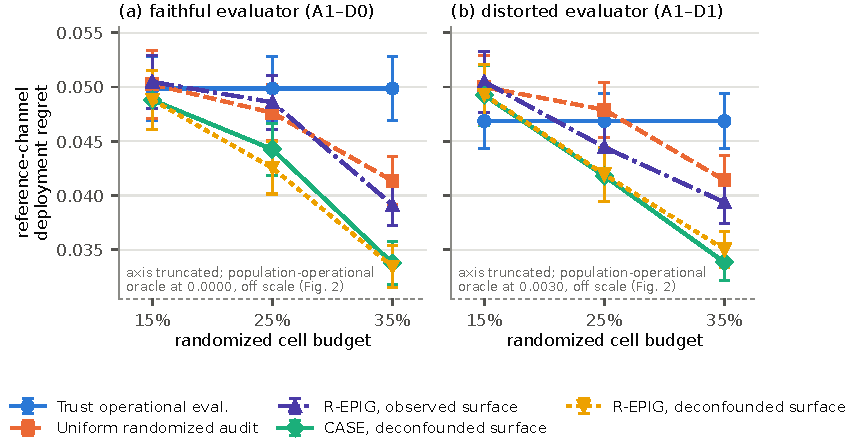
\includegraphics[width=\textwidth]{figs/tae_fig1.pdf}
\caption{\textbf{Deconfounding the acquisition surface matters more than the rule that spends the
budget.} Deployment regret (lower is better) under the selective-router log, with error bars giving
paired standard errors over $30$ partitions. The two deconfounded-surface arms track each other and
sit below the surface-agnostic uniform rule and the observed-surface rule, and they buy $86\%$ of the
same cells (Q3). \textbf{The main axis is truncated} so that the methods, which span $0.033$
to $0.051$, are legible, and the inset in each panel repeats trust and CASE on the full axis with
both oracles, so the spread between the methods can be read against the much larger gap that
separates all of them from a perfect repair. Per-slice values appear in Fig.~\ref{fig:fig3} and
Table~\ref{tab:slices}.}
\label{fig:fig1}
\end{figure}

\subsection{Core validity results}\label{sec:core}

\paragraph{Q1. The log names the wrong model in two thirds of request types.} Under A1--D0 the logged
surface picks a model other than the target-best one in $67.5\%\se{2.4}$ of contexts, against
$39.6\%\se{2.6}$ for the matched-volume common-population log. In regret the figures are
$0.0499\se{0.0030}$ against $0.0214\se{0.0024}$. The gap is selection rather than sample size, because
the two logs hold the same requests in the same per-cell counts, and no outcome oracle enters A1. On
RouterBench the same statistics are $46.9\%\se{3.3}$ and $25.6\%\se{2.9}$.

\paragraph{Q2. Auditing repairs a substantial fraction, and no more.} At a $35\%$ budget under
A1--D0, CASE lowers regret from $0.0499\se{0.0030}$ to $0.0338\se{0.0020}$, a paired difference of
$-0.0161$ with $95\%$ CI $[-0.0219,-0.0103]$, better on $27$ of $30$ partitions and excluding zero
under all three resampling schemes of App.~\ref{app:ci}. It improves on all five slices, and on
RouterBench the effect is larger, from $0.0784$ to $0.0421$, a paired difference of
$-0.0363\se{0.0042}$ better on \emph{every} partition. How far this goes towards a perfect repair
depends on the estimand, so we give both. The mean over partitions of the per-partition share of the
trust-to-oracle gap that CASE closes is $28\%$, and the share formed from aggregate means is
$32\%$.

\emph{Why only a third?} Not the budget. Prop.~\ref{prop:decomp} is cellwise but the deployed
correction is one offset per model, and the router makes that misspecified, since $68\%\se{2}$ of the
selection distortion is not constant across contexts. Replacing the budget-limited fit with the
\emph{best-fitting member of the same family}, computed from the truth with no budget at all, reaches
$0.0318\se{0.0025}$, only $0.0020\se{0.0024}$ below CASE with $95\%$ CI $[-0.0030,+0.0070]$. So of the
trust-to-oracle gap, CASE closes the $28\%$ above, a further $5\%$ is reachable inside the
action-level family ($14\%$ at the top of that interval), and roughly two thirds lies outside it, all
three shares being mean-of-ratios over partitions. More readouts would not help, whereas a richer
corrector would, but the richer families we tried overfit $13$ purchased cells
(App.~\ref{app:extra}).

\paragraph{Q3. The surface decides more than the rule, but the rule is not free.} Crossing the
acquisition rule (smallest-margin against decision-information) with the acquisition surface
(observed against deconfounded) separates the two. \emph{Holding the rule fixed, moving to the
deconfounded surface helps in all eight cells across both corpora}, by $0.0036$ to $0.0115$. Holding
the surface fixed, the rule ties on the five-model corpus, with a paired difference of
$+0.0003\se{0.0011}$ and two one-sided tests rejecting a difference larger than $0.005$ at
$p=10^{-4}$. The two rules also buy $86.5\%\se{1.0}$ of the same cells, against $61.4\%\se{1.0}$ when
the same rule moves to the observed surface, so the tie is mechanical rather than coincidental.
\textbf{On the eleven-model corpus the rule does matter, and the margin heuristic loses to the
decision-information rule by $+0.0140\se{0.0021}$.} The bounded claim is that deconfounding the
surface is the robust lever and that a simple margin rule becomes inadequate as the roster grows.

\begin{figure}[t]\centering
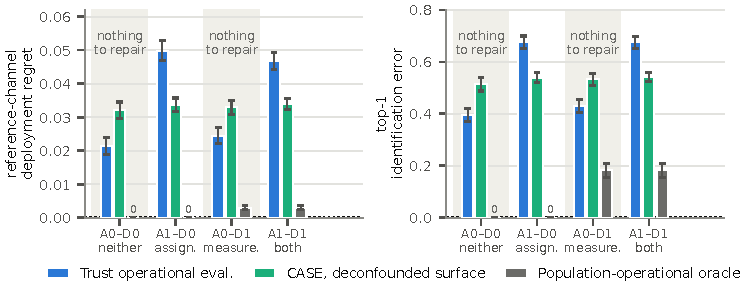
\includegraphics[width=\textwidth]{figs/tae_fig2.pdf}
\caption{\textbf{The four-cell decomposition} at a $35\%$ budget, where the reference-outcome oracle
is $0$ in every cell by construction. Shaded cells have no assignment invalidity to repair, so CASE
sitting \emph{above} trust there is the variance cost of buying $30$-request readouts rather than a
failure of the method (Q6). In the both-failures cell, the part of the logged loss a cellwise-perfect
repair removes is $\Gsel=0.0439\se{0.0029}$, and the measurement floor that survives it is
$\Gmeas=0.0030$ in regret but $18.3\%\se{2.7}$ in identification error.}
\label{fig:fig2}
\end{figure}

\paragraph{Q4. None of it buys measurement validity.} In the both-failures cell the logged evaluation
loses $0.0469\se{0.0025}$. A cellwise-perfect repair removes $\Gsel=0.0439\se{0.0029}$ and leaves
$\Gmeas=0.0030$, with $95\%$ CI $[+0.0017,+0.0043]$ over partitions, though it is \emph{not} separable
from zero when the five slices are resampled as clusters (App.~\ref{app:ci}). The measurement-only
cell makes the point with no selection bias to repair, since CASE sits at $0.0330\se{0.0021}$
against $0.0030\se{0.0006}$ for the population-operational oracle.

The floor is small in \emph{value} and large in \emph{identification}. With selection bias removed
exactly, the evaluator still names the wrong model in $18.3\%\se{2.7}$ of contexts on the primary
corpus and $13.8\%\se{1.5}$ on RouterBench, both at the pre-specified distortion strength and
$J{=}8$. Across every sensitivity we ran the floor spans $10.0$ to $30.6\%$, at its lowest under a
context-invariant model preference and its highest at twice the pre-specified distortion
(App.~\ref{app:extra}), so the headline pair is a point inside a range rather than a constant.
Reversals concentrate where the target margin is smallest, so they are cheap in regret and expensive
in ranking, and the two reports disagree by an order of magnitude about what this evaluator's bias
costs. \textbf{We stress what this number is and is not.} Applying Cor.~\ref{cor:margin} to the
margin distribution alone, with no reference to which model actually wins, predicts $28.8\%\se{2.7}$
against the $18.3\%\se{2.7}$ observed, so the rate is largely fixed by $\lambda$ and the margins and
carries \emph{no} information about how biased any deployed judge is. What is not arithmetic is the
structural claim it illustrates, that a cellwise-perfect assignment repair leaves this error
untouched.

\subsection{Practical deployment questions}\label{sec:practical}

\paragraph{Q5. A same-evaluator check cuts harm but cannot validate the construct, and gating pays
only under an asymmetry.} Both held-out checks cut harmful switches, from $0.178\se{0.030}$ ungated
to $0.061\se{0.019}$ for the same evaluator and $0.072\se{0.021}$ for the reference channel
(Table~\ref{tab:deploy}). \textbf{We had pre-specified that the same-evaluator check would leave
\emph{more} harmful switches, and it does not.} It is correlated with the baseline it checks, because
the log-derived policy is the argmax of the operational surface, so reading verification through the
same distortion tilts toward retention. At the stronger bias level it switches less ($0.55$ against
$0.62$) and falsely retains more ($0.242\se{0.035}$ against $0.208\se{0.032}$). What it provably
cannot do is get the verdict right. On $4.6\%$ of contested contexts, or $8.3\%$ at the stronger
level, its \emph{population} comparison points the opposite way from the target's, a property of the
channel rather than the sample, unchanged by budget and flat in readout size.

Gating is not free. It trades $0.117$ fewer false switches for $0.233$ more false retentions, so it
lowers expected loss only if a harmful switch costs at least $2.0\times$ a missed improvement at the
$35\%$ budget, and $1.0\times$ at the $15\%$ budget, where the audit behind it is too thin to trust
(App.~\ref{app:extra}). \emph{State the asymmetry before quoting the gate.}

\paragraph{Q6. You can tell in advance whether the audit is worth buying.} Where the log is already
common-population and its cells are larger than the readouts that would replace them, auditing
\emph{raises} regret, from $0.0214\se{0.0024}$ to $0.0321\se{0.0024}$ (paired $+0.0107$, CI
$[+0.0067,+0.0147]$, not separable from zero under slice resampling), because each $30$-request
readout is noisier than the ${\approx}140$-request log cell it overwrites. The binding condition is
that density comparison rather than the audit itself, and on RouterBench, whose log cells are far
larger, the cost disappears ($-0.0005\se{0.0037}$). A test makes
this actionable. After just the $K$ per-model seed readouts, take the dispersion of the
logged-minus-audit differences, standardised by the noise they would carry under a common-population
log. It averages $1.06\se{0.03}$ under A0 and $1.28\se{0.04}$ under A1, with AUC
$0.79$, and auditing only above a threshold gives mean regret $0.0313$ against $0.0329$ for always
auditing and $0.0356$ for never auditing. The threshold is fitted in-sample, so the AUC is the honest
separation, but five cells can inform the decision rather than leaving it blind.

% =============================================================================
\section{Conclusion}\label{sec:scope}
% =============================================================================
A logged model comparison can fail in two ways that call for different remedies. Randomized auditing
repairs the assignment failure under stated conditions, removing between a quarter and a third of the
distance to a perfect repair on the primary corpus and rather more on the second. It does not repair the
measurement failure at all. Once selection bias is removed exactly, the evaluator still names the
wrong model in $14$ to $18\%$ of request types on the two corpora at the pre-specified distortion
strength, and in $10$ to $31\%$ across our sensitivity analyses, in every case whatever the audit
budget. Three further results are
practical. What makes a budget productive is the surface it is spent on rather than the rule that
spends it, though the rule regains importance as the roster grows. A held-out check reduces harmful
deployment changes but inherits the construct it was meant to check, and pays only when a harmful
switch costs roughly twice a missed improvement. And the first few randomized measurements already
indicate whether a larger audit is worth buying, which matters where the readouts would be thinner
than the log cells they overwrite. That cost, $+0.0107$ on the primary corpus and not separable from
zero once benchmark slices are resampled as clusters, is a statement about readout size relative to
log-cell density rather than about auditing as such, and it disappears on RouterBench, whose log
cells are far larger.

\begin{table}[t]\centering\footnotesize\setlength{\tabcolsep}{5pt}
\caption{Validity scope of a randomized audit over a router-generated log.}
\label{tab:scope}
\begin{tabular}{@{}lll@{}}
\toprule
Threat & Addressed? & Required condition\\
\midrule
Router-induced selective assignment & Yes, partly & Randomizable cells, correction family rich enough\\
Finite audit noise & Partially & Readouts no thinner than the log cells they replace (Q6)\\
Context-varying selection residual & \textbf{Largely not} & Two thirds of it lies outside the fitted family\\
Stable shared evaluator distortion & \textbf{No} & Construct validation or a \emph{validated} channel\\
Evaluator error that depends on the request & Can contaminate & Assignment invariance (Prop.~\ref{prop:decomp}a)\\
Unsupported model--context cells & No & Exploration or expanded support\\
\bottomrule
\end{tabular}
\end{table}

\paragraph{Limitations.} Table~\ref{tab:scope} lists what the protocol addresses, and two limitations matter most. The
identification result of \S\ref{sec:model} holds for any evaluator, but the magnitudes come from a
pre-specified synthetic distortion rather than a measured judge, so nothing here estimates construct
bias for a deployed LLM judge, and measuring that is the natural next step. The reference channel
reads the designated target during verification, an experimental control rather than something a
production team can obtain on demand, so it bounds what a better channel could achieve rather than
describing an available one.

\paragraph{A reporting checklist.} A comparison read off a router-generated log should report (i)
the assignment mechanism and the per-cell logged counts, (ii) which evaluator scored each stream and whether its error is plausibly invariant to
routing, not merely that the same judge was used, (iii) the outcome the conclusion is \emph{about}
and how it differs from what was measured, (iv) the target margin per context beside the ranking, so
Cor.~\ref{cor:margin} is checkable, and (v) both a value and an identification metric, which can
disagree by an order of magnitude.

\label{endofmaintext}
\bibliographystyle{plainnat}
\bibliography{tae_refs}

\appendix
\newpage
% =============================================================================
\section{Proofs}\label{app:proof}
% =============================================================================
\begin{proof}[Proof of Prop.~\ref{prop:decomp}]
Write the operational score as the target plus an error, $\widetilde Y^s_i(k)=\Yref_i(k)+e^s_i(k)$.
Conditioning on the logged assignment and adding and subtracting $\muref_{kj}$,
\[
M_{kj}=\mathbb E\!\left[\Yref_i(k)\mid A_i{=}k,Z_i{=}j\right]
      +\mathbb E\!\left[e^o_i(k)\mid A_i{=}k,Z_i{=}j\right]
=\muref_{kj}+\Bsel_{kj}+C^{o,\mathrm{sel}}_{kj}.
\]
The audit readout draws context-$j$ requests at random, so
$R_{kj}=\muref_{kj}+C^{i,\mathrm{pop}}_{kj}$. Subtracting gives
$M_{kj}-R_{kj}=\Bsel_{kj}+(C^{o,\mathrm{sel}}_{kj}-C^{i,\mathrm{pop}}_{kj})$, which recovers
$\Bsel_{kj}$ if and only if the bracket vanishes, giving part (a). Note what (a) does \emph{not} say.
Using the same evaluator on both streams equates the two error \emph{functions}, $e^o=e^i$, but not
the two conditional means, and those means are taken over different populations whenever the router
selects within a context.

For (b), suppose additionally that the error depends on the request only through its cell, so that
$\mathbb E[e^s_i(k)\mid \mathcal E,Z_i{=}j]=C_{kj}$ for every conditioning event $\mathcal E$ within
context $j$. Then $C^{o,\mathrm{sel}}_{kj}=C^{i,\mathrm{pop}}_{kj}=C_{kj}$, the recovered difference
is $\Bsel_{kj}$, and removing it from $M_{kj}=\muref_{kj}+\Bsel_{kj}+C_{kj}$ leaves
$\muref_{kj}+C_{kj}=\muop_{kj}$. If moreover $C_{kj}=C_k$ for all $j$, then $C_k$ never enters
$M_{kj}-R_{kj}$ at all, so no differencing estimator can see it while $\muop_{kj}$ retains it, and a
per-model correction fitted from the differences therefore cannot remove it. App.~\ref{app:extra}
instantiates exactly this case.
\end{proof}

\begin{proof}[Proof of Cor.~\ref{cor:margin}]
Write $k^\star=\piref(j)$. The deployed policy picks $k^\star$ if and only if for every
$k\neq k^\star$, $\muref_{k^\star j}+\varepsilon_{k^\star j}>\muref_{kj}+\varepsilon_{kj}$, that is,
$\varepsilon_{kj}-\varepsilon_{k^\star j}<\muref_{k^\star j}-\muref_{kj}$. The right-hand side is at
least $\Delta_j$, which gives the stated condition, and
$\varepsilon_{kj}-\varepsilon_{k^\star j}\leq 2\max_k|\varepsilon_{kj}|$ gives the sufficient form.
\end{proof}

\begin{remark}[Why the reversals are cheap]\label{rem:cheap}
Cor.~\ref{cor:margin} implies that with distortion bounded by $\epsilon$, only contexts with
$\Delta_j<2\epsilon$ can flip, and each flip costs at most $\Delta_j<2\epsilon$. This is the pattern
\S\ref{sec:results} reports, in which many contexts flip but the regret cost is an order of magnitude
below a distortion-sized loss per flipped context.
\end{remark}

% =============================================================================
\section{Leakage and algebra tests}\label{app:tests}
% =============================================================================
\paragraph{Reproducibility.} Anonymized supplementary material accompanies the submission, containing
the experiment package, the pre-registered analysis plan, all tests below, and the long-form result
files behind every number. It regenerates in minutes and uses only released per-request benchmark
outputs, with no new model inference. The result files key the evaluator factor E where the paper
writes D, and the mapping is recorded in the supplementary claim registry.

All six tests run before any result file is written, and the runner exits non-zero if one fails.
Values are from partition $0$ of the primary corpus, and all $30$ partitions pass.

\begin{enumerate}[leftmargin=1.4em,itemsep=1pt,topsep=2pt]
\item \textbf{Cohort isolation.} The five cohorts are pairwise disjoint and exhaust the $11{,}289$
requests.
\item \textbf{Assignment matching.} A paired A0/A1 run has identical per-cell counts, identical total
log volume ($5{,}644$ requests) and identical evaluator distortion, and every A0 cell draws only from
its own context's log cohort.
\item \textbf{Reference-channel leakage.} Replacing the scoring cohort's target outcomes with uniform
random values leaves the acquired cells, the fitted correction, the deployed surface (max difference
$0.0$), the candidate policy and the gate decision identical. The allocator is called with the scoring
surface set to \texttt{None}, so reading it would raise rather than bias.
\item \textbf{Stable-evaluator algebra.} With $C^o=C^i$ the logged-minus-audit difference is unchanged
by the distortion (mean absolute change $0.0019$ against an effective distortion of $0.0121$), while
the population-operational surface differs from the target surface by exactly that distortion.
Clipping attenuates the nominal distortion by $0.476\se{0.003}$.
\item \textbf{Assignment invariance} (Prop.~\ref{prop:decomp}(a)). The residual
$|C^{o,\mathrm{sel}}-C^{i,\mathrm{pop}}|$ is measured rather than assumed. It is $0.0018\se{0.0001}$
over $30$ partitions, against a cohort-sampling floor of $0.0013\se{0.0001}$ with routing removed and
a selection bias of $0.0991\se{0.0019}$, so contamination is $1.8\%\se{0.1}$. Twice the residual is
$0.0036$, an order of magnitude below the $0.041$ median target margin, so by Cor.~\ref{cor:margin} it
cannot flip a typical context. It is non-zero because clipping makes the realised per-request error
depend on the request's own target outcome, which the router selects on.
\item \textbf{Stream-mismatch algebra.} With $C^i=\tfrac12C^o$ the estimated cellwise difference gains
the predicted extra term, with correlation $0.94$ against $\tfrac12C^o$ and slope $0.46$, the clipping
attenuation.
\end{enumerate}

% =============================================================================
\section{Additional results}\label{app:extra}
% =============================================================================
Each subsection sets out the question that motivated the analysis, the factor that was varied, and
the finding, followed by the supporting table or figure.

\subsection{The four validity cells in one table}
The main text quotes individual cells of the factorial, but a reader checking the decomposition needs
all four together, with every arm, on one scale. Table~\ref{tab:factorial} gives all six arms at the
$35\%$ budget in each of the four cells, over $30$ partitions crossed with $6$ acquisition seeds. The
pattern the paper argues for is then visible in one place. Auditing helps only where assignment
invalidity is present, which is the contrast between the A1 rows and the A0 rows, and the
population-operational oracle is zero under a faithful evaluator but not under a distorted one.

\begin{table}[h]\centering\small\setlength{\tabcolsep}{3.6pt}
\caption{Deployment regret at a $35\%$ budget, all four validity cells, primary corpus, with $\pm$ a
paired SE over $30$ partitions.}
\label{tab:factorial}
\begin{tabular}{@{}lcccccc@{}}
\toprule
Cell & Trust & Uniform & CASE & R-EPIG$_{\mathrm{corr}}$ & Pop.-op.\ oracle & Ref.\ oracle\\
\midrule
\TAEfactorialrows
\bottomrule
\end{tabular}
\end{table}

\subsection{Does the result come from one benchmark slice?}
A pooled improvement can be produced by a single slice while the others are flat or worse, in which
case it would not be a general finding. To check this we re-score the pooled deployed policy on each
slice's scoring requests separately, against the pooled target policy. The audit improves on all five
slices rather than on one, although the size varies by roughly a factor of ten between MMLU-Pro and
ArenaHard, which is why the slice-cluster interval in App.~\ref{app:ci} is much wider than the
partition interval.

\begin{figure}[h]\centering
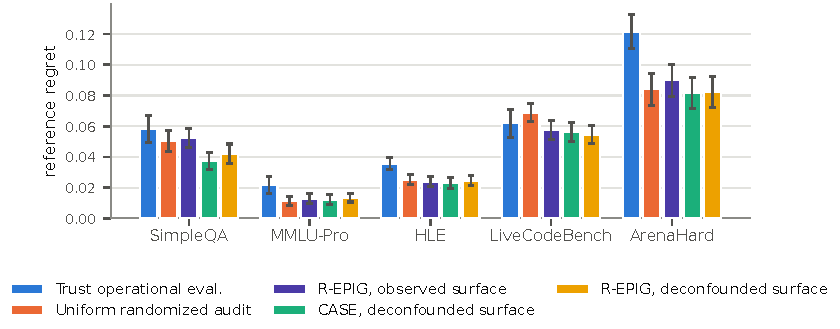
\includegraphics[width=\textwidth]{figs/tae_fig3.pdf}
\caption{Slice contributions to the pooled-policy regret at a $35\%$ budget under A1--D1, the
per-slice view of Fig.~\ref{fig:fig1}. Values are in Table~\ref{tab:slices}.}
\label{fig:fig3}
\end{figure}

\begin{table}[h]\centering\footnotesize\setlength{\tabcolsep}{3.4pt}
\caption{\textbf{Slice contributions to pooled-policy regret} at a $35\%$ budget under the
selective-router log. Each entry evaluates the \emph{pooled} deployed policy on that slice's scoring
requests only, against the pooled target policy, so an entry can be slightly negative when a slice's
sub-population within a mixed context prefers a different model. The last column is the unweighted
average over slices. It is a different estimator from the pooled regret of Table~\ref{tab:factorial}
and the two should not be compared numerically.}
\label{tab:slices}
\begin{tabular}{@{}lcccccc@{}}
\toprule
Method & SimpleQA & MMLU-Pro & HLE & LiveCodeBench & ArenaHard & Unwtd.\ avg.\\
\midrule
\TAEslicerows
\bottomrule
\end{tabular}
\end{table}

\subsection{What happens when the audit result is actually deployed}
Lower regret does not by itself mean a team should act on the audit, because acting means replacing
whatever the log currently recommends, and that change can be harmful. We therefore compare three
arms at matched total budget, deploying the audited candidate ungated and gating it on a held-out
check read either by the operational evaluator or by the target channel. Both checks cut harmful
switches by roughly two thirds and are indistinguishable from each other on that outcome, but only
the target channel has a verdict that is right in the limit.

\begin{table}[h]\centering\small\setlength{\tabcolsep}{4.4pt}
\caption{\textbf{Deployment decisions at matched total budget} ($35\%$, where every row spends $13$
cells and gated rows move $4$ to verification). A \emph{false switch} replaces the log-derived
deployment policy ($\arg\max_k M_{kj}$, \emph{not} the incumbent router) with the audited candidate
when the candidate has strictly lower target value on the untouched scoring cohort, and \emph{false
retention} is the converse. \emph{Verdict inversion} is the fraction of contested contexts on which
the checking channel's \emph{population} comparison disagrees with the target's, a systematic error no
budget removes.}
\label{tab:deploy}
\begin{tabular}{@{}lcccccc@{}}
\toprule
& Ref.\ regret & False switch & False retention & Switch & Cells & Verdict\\
& $\downarrow$ & $\downarrow$ & $\downarrow$ & rate & acq.\,/\,ver. & inversion\\
\midrule
\TAEdeploymentrows
\bottomrule
\end{tabular}
\end{table}

\subsection{Does any of this survive a different benchmark and a different model roster?}
Every number above comes from one corpus, so its intervals describe that corpus rather than routing
in general. We therefore run the identical pipeline, with the same cohorts, contexts, router,
distortion formula, methods and budgets, on RouterBench, which holds $36{,}497$ requests and $11$
models across five benchmark families and shares no requests, models or scoring convention with the
primary corpus. Three findings replicate and two do not, and we report both outcomes.

Selection is present, since the log misranks $46.9\%\se{3.3}$ of contexts against $25.6\%\se{2.9}$
for the matched common-population log. Auditing repairs part of it, taking A1--D0 trust from $0.0784$
to CASE at $0.0421$, a paired $-0.0363\se{0.0042}$ that is better on every partition. A
cellwise-perfect repair still leaves a measurement floor of $13.8\%\se{1.5}$ identification error and
$0.0053$ regret. The two findings that do not replicate are corpus-specific. First, the rule tie does
not, because with $11$ models the margin heuristic loses to the decision-information rule by
$+0.0140\se{0.0021}$ (A1--D0) and $+0.0066\se{0.0027}$ (A1--D1). Second, the cost of auditing under a
common-population log does not, because here CASE minus trust is $-0.0005\se{0.0037}$ rather than
$+0.0107$, consistent with RouterBench's much larger log cells leaving less variance for a
$30$-request readout to add.

\begin{center}\footnotesize
\begin{tabular}{@{}llcc@{}}
\toprule
Acquisition rule & Corpus & Observed surface & Deconfounded surface\\
\midrule
Smallest margin & LLMRouterBench ($K{=}5$) & $0.0402\se{0.0019}$ & $0.0338\se{0.0020}$\\
Decision-information & LLMRouterBench ($K{=}5$) & $0.0391\se{0.0019}$ & $0.0335\se{0.0019}$\\
Smallest margin & RouterBench ($K{=}11$) & $0.0467\se{0.0030}$ & $0.0421\se{0.0036}$\\
Decision-information & RouterBench ($K{=}11$) & $0.0396\se{0.0023}$ & $0.0281\se{0.0029}$\\
\bottomrule
\end{tabular}
\end{center}
\noindent A1--D0 at a $35\%$ budget. The surface effect is negative in all four rows and in the
matching D1 rows, while the rule effect is null at $K{=}5$ and large at $K{=}11$.

\subsection{Is the un-repaired gap a budget problem or a model problem?}
CASE closes between a quarter and a third of the distance to a perfect repair, and a reader is
entitled to ask whether the rest would come with more readouts. To separate the two explanations we hold CASE's
allocation and budget fixed and vary only the correction, adding shrinkage, a two-way additive fit
and a rank-2 completion, together with \textsc{oracle row}, the best-fitting correction inside the
same one-offset per-model family computed from the truth with no budget at all. That last arm is the
family's least-squares optimum rather than its regret optimum, so it estimates the ceiling rather
than bounding it. The answer is that the shortfall is a model problem. The no-budget ceiling is
$0.0318\se{0.0025}$, within noise of what CASE already achieves, so more readouts would buy almost
nothing, while the richer families overfit the $13$ purchased cells and do worse.

\begin{center}\footnotesize
\begin{tabular}{@{}lcc@{}}
\toprule
Correction, at CASE's allocation and a $35\%$ budget & A1--D0 & A1--D1\\
\midrule
Trust the log (no correction) & $0.0499\se{0.0030}$ & $0.0469\se{0.0025}$\\
Action-level (deployed) & $0.0338\se{0.0020}$ & $0.0338\se{0.0017}$\\
\;+ experiment-grounded shrinkage \citep{athey2020combining} & $0.0339\se{0.0020}$ & $0.0338\se{0.0017}$\\
Two-way additive (row $+$ column) & $0.0399\se{0.0019}$ & $0.0394\se{0.0024}$\\
Rank-2 completion of the purchased bias residuals & $0.0452\se{0.0019}$ & $0.0426\se{0.0019}$\\
\addlinespace[2pt]
\textsc{oracle row}: best-fitting action-level correction, no budget & $0.0318\se{0.0025}$ & $0.0337\se{0.0024}$\\
\textsc{oracle cell}: population-operational surface & $0.0000$ & $0.0030\se{0.0006}$\\
\bottomrule
\end{tabular}
\end{center}
\noindent $30$ partitions crossed with $6$ seeds. Diagnostics: $68.4\%\se{2.0}$ of the selection
distortion is not row-constant, the within-row standard deviation is $0.101\se{0.003}$, and the
fitted offsets differ from the best-fitting ones by $0.079\se{0.003}$. CASE minus \textsc{oracle row}
is $+0.0020\se{0.0024}$, and two one-sided tests do \emph{not} establish equivalence at a $0.005$
margin ($p=0.11$), so we report the $95\%$ CI $[-0.0030,+0.0070]$ rather than claiming a tie.

\subsection{When is a deployment gate worth using?}
A gate trades one kind of mistake for another, so calling it a safety measure is incomplete without
saying how the two mistakes compare in cost. We therefore compute, at each budget, the ratio
$c^\star=\Delta\text{retention}/|\Delta\text{switch}|$ above which gating lowers expected loss, which
gives a usable rule of thumb. Under A1--D1, $c^\star=0.98$ at a $15\%$
budget, $1.64$ at $25\%$ and $2.00$ at $35\%$, and for the reference channel $1.03$, $1.40$ and
$2.21$. Gating also changes regret by $-0.0051$, $+0.0021$ and $+0.0036$ respectively, so it earns
its cells when the audit behind it is thin and costs value when the audit is rich.

\subsection{Are the two claimed ties really ties?}
A difference that fails to reach significance is not the same as a demonstrated equivalence, and the
paper leans on two such claims. We therefore report the minimum detectable paired difference at $30$
partitions and run two one-sided tests against a margin fixed in advance at $0.005$, a tenth of the
loss of trusting the log. One claim survives as a genuine equivalence and one does not. The minimum
detectable difference is $0.0031$ for the CASE against
R-EPIG$_{\mathrm{corr}}$ contrast, and the two one-sided tests give $p=1\times10^{-4}$ (A1--D0) and
$p=8\times10^{-4}$ (A1--D1), so the two rules are equivalent at that margin. The same test does not
establish equivalence between CASE and the action-level ceiling, which is why that comparison is
reported above as an interval rather than a tie.

\subsection{Can a team tell in advance whether to audit?}
The result that auditing a balanced log adds error is only actionable if the imbalance can be
detected before the budget is spent. From the $K$ per-model seed readouts alone, which every arm buys
first, we take the dispersion of $M_{kj}-R_{kj}$ standardised by the noise it would carry if the log
were common-population. This separates the two regimes and yields a decision rule that beats both
fixed policies. The statistic averages $1.06\se{0.03}$ under A0 and
$1.28\se{0.04}$ under A1, with AUC $0.79$, a best in-sample threshold of $1.17$ and accuracy $75\%$.
Auditing only above that threshold gives mean regret $0.0313$, against $0.0329$ for always auditing
and $0.0356$ for never auditing.

\subsection{How much does the result depend on how aggressively the router selects?}
Assignment validity is half the paper, and its magnitude is set entirely by how sharply the incumbent
router selects, which the main runs fix at an exploration rate of $0.15$. We sweep that rate, since
$\varepsilon\to1$ is uniform routing and reproduces A0 by construction. Both the damage and the
repair scale with the selection, which is what the mechanism predicts and what makes an audit worth
buying only where selection is present.

\begin{center}\footnotesize
\begin{tabular}{@{}lcccc@{}}
\toprule
Exploration rate $\varepsilon$ & $0.05$ & $0.15$ & $0.30$ & $0.50$\\
\midrule
Log top-1 error, A1--D0 & $0.631$ & $0.675$ & $0.613$ & $0.569$\\
Trust the log & $0.0476$ & $0.0499$ & $0.0412$ & $0.0368$\\
CASE & $0.0292$ & $0.0338$ & $0.0344$ & $0.0333$\\
R-EPIG, deconfounded surface & $0.0282$ & $0.0335$ & $0.0330$ & $0.0334$\\
\addlinespace[2pt]
CASE $-$ trust & $-0.0183\se{0.0041}$ & $-0.0161\se{0.0028}$ & $-0.0068\se{0.0044}$ & $-0.0035\se{0.0036}$\\
Share of the trust regret removed & $39\%$ & $32\%$ & $17\%$ & $10\%$\\
\bottomrule
\end{tabular}
\end{center}
\noindent A1--D0 at a $35\%$ budget over $20$ partitions crossed with $6$ seeds, with
$\varepsilon=0.15$ taken from the main runs. The repair falls monotonically as the router explores
more, from $39\%$ of the trust regret at $\varepsilon=0.05$ to $10\%$ at $\varepsilon=0.50$. The
damage is not monotone at the sharpest setting, and the reason is support rather than bias. At
$\varepsilon=0.05$ only $28.6$ of the $40$ model--context cells appear in the log at all, against
$36.2$ at $\varepsilon=0.15$ and $40.0$ at $\varepsilon=0.50$, and a cell that never appears is
excluded from the comparison, so the surviving comparison is both smaller and easier. Aggressive
routing therefore converts part of the bias problem into the support problem the last row of
Table~\ref{tab:scope} records, which no audit budget addresses. What this sweep does not vary is the
router \emph{family}, which remains a cost cascade throughout.

\subsection{How much does the result depend on the shape and size of the distortion?}
The evaluator distortion is a modelling choice, so a result that only holds at one strength or one
functional form would be an artefact of that choice. We therefore vary the strength to the
pre-specified stronger level, replace the capability-by-difficulty interaction with a
context-invariant model preference, and reverse the sign of the mismatch between the log and audit
streams. The measurement result holds in every variant, while the mismatch result turns out not to
have a stable direction.

At $\lambda=1.0\times$ the training median margin the reversal rate rises from $18.3\%$ to $30.6\%$
and the floor from $0.0030$ to $0.0069\se{0.0014}$, while CASE's regret is unchanged at
$0.0333\se{0.0026}$, and the same-evaluator gate's verdict-inversion rate rises to $8.3\%\se{1.9}$.
Setting $C_{kj}=C_k$, a judge that simply prefers some models everywhere and the cleanest case of
Prop.~\ref{prop:decomp}(b), cancels from the differencing entirely, yet a cellwise-perfect repair
still misidentifies $10.0\%\se{2.1}$ of contexts, so the measurement result does not depend on the
capability-by-difficulty interaction. With $C^i=-\tfrac12C^o$ CASE reaches $0.0313\se{0.0021}$, so
attenuation slightly worsens regret and sign reversal slightly improves it, and mismatch is real in
the algebra but not directionally stable.

\subsection{How much does the result depend on the experimental settings?}
Three settings were chosen rather than derived, namely how many requests each purchased cell reads,
how finely requests are grouped into contexts, and which policy counts as the status quo. We sweep
the readout size, the number of contexts, and the definition of the baseline the gate compares
against. Every qualitative conclusion is stable, while two magnitudes are not, which is why the main
text reports the identification floor as the top of a range.

With $n\in\{15,30,60\}$ CASE reaches $0.0365$, $0.0338$ and $0.0338$, and the verdict-inversion rate
is flat at $6.0\%$, $4.6\%$ and $5.8\%$, as a systematic error must be. Across $J\in\{6,8,12,16\}$ the
log misranks about two thirds of contexts, the audit reduces regret, the two deconfounded rules track
each other, and a cellwise-perfect repair leaves a non-zero floor, while the identification floor
ranges over $10.4$ to $18.3\%$. Taking the \emph{incumbent router} rather than the log-derived policy
as the status quo makes switching almost always beneficial (ungated false switch $0.058\se{0.022}$),
so that comparison is uninformative, and the main text uses the log-derived baseline because the
question is whether an evaluation \emph{conclusion} supports a change.

% =============================================================================
\section{Confidence intervals for the confirmatory contrasts}\label{app:ci}
% =============================================================================
The $\pm$ used elsewhere is a paired standard error over the $30$ partitions, which answers one
question, namely whether a different split and acquisition draw would agree, and not two others.
\emph{Partition} is a paired $t$ interval over partitions. \emph{Request} is a nonparametric bootstrap
of the scoring cohort, $2000$ replicates with common random numbers, each run's deployed policy held
fixed while $\muref$ and $\piref$ are re-estimated per replicate. \emph{Slice} is a cluster bootstrap
over the five benchmark slices, $10^4$ replicates. Five clusters make it coarse and wide by
construction, and it is the closest thing here to asking whether a result would survive a different
suite.

\begin{center}\scriptsize\setlength{\tabcolsep}{3.2pt}
\begin{tabular}{@{}lrccc@{}}
\toprule
Contrast ($35\%$ budget) & Mean & Partition & Request & Slice clusters\\
\midrule
A1--D0: CASE $-$ trust & $-0.0161$ & $[-.0219,-.0103]$ & $[-.0190,-.0132]$ & $[-.0410,-.0083]$\\
A1--D0: CASE $-$ R-EPIG$_{\mathrm{corr}}$ & $+0.0003$ & $[-.0019,+.0025]$ & $[-.0007,+.0013]$ & $[-.0017,+.0007]$\\
A1--D1: CASE $-$ trust & $-0.0130$ & $[-.0179,-.0081]$ & $[-.0159,-.0103]$ & $[-.0293,-.0087]$\\
A1--D1: CASE $-$ pop.-operational oracle & $+0.0309$ & $[+.0271,+.0346]$ & $[+.0278,+.0338]$ & $[+.0193,+.0444]$\\
A1--D1: measurement floor $\Gmeas$ & $+0.0030$ & $[+.0017,+.0043]$ & $[+.0011,+.0047]$ & $\mathbf{[-.0002,+.0259]}$\\
A0--D0: CASE $-$ trust (cost of auditing) & $+0.0107$ & $[+.0067,+.0147]$ & $[+.0083,+.0132]$ & $\mathbf{[-.0013,+.0142]}$\\
\addlinespace[2pt]
A1--D1: false switch, same $-$ ref.\ channel & $-0.0111$ & $[-.0269,+.0047]$ & --- & ---\\
A1--D2: false switch, same $-$ ref.\ channel & $-0.0278$ & $[-.0514,-.0042]$ & --- & ---\\
\bottomrule
\end{tabular}
\end{center}
\noindent\emph{Leading zeros are dropped inside the intervals.}

Three conclusions are unaffected by the scheme. The audit benefit under both evaluator conditions
excludes zero everywhere, slice resampling included, so it is not carried by one benchmark. The CASE
against R-EPIG tie is tight under all three, with a widest interval of $[-.0017,+.0007]$. And CASE's
distance from the population-operational oracle stays large and positive. Two conclusions are weaker
than the partition interval alone suggests, and the main text flags both. The measurement floor
\emph{in value} and the cost of auditing under A0 each lose separation from zero under the five-slice
cluster bootstrap. Neither is surprising, given small quantities and five clusters, but neither should
be quoted as established across benchmark suites. The identification-side floor does not depend on
this.

\end{document}
